%!TEX root = RJwrapper.tex
\title{\pkg{RNGforGPD}: An R Package for Generation of Univariate and Multivariate Generalized Poisson Data}
\author{by Hesen Li, Hakan Demirtas, and Ruizhe Chen}

\maketitle

\abstract{
This article describes the R package \pkg{RNGforGPD}, which is designed for the generation of univariate and multivariate generalized Poisson data. Some illustrative examples are given, the utility and functionality of the package are demonstrated; and its performance is assessed via simulations that are devised around both artificial and real data.
}

\section{Introduction and motivation}

It is well known that the variance of a Poisson variable equals to its mean. However, over- and under- dispersion in count data could make this mean-variance equality assumption unrealistically simplistic. This situation is often caused by the heterogeneity in the population, while we implicitly assume that the weights assigned to each event are equal when we employ the regular Poisson distribution. This problem can be addressed by modeling count data using the generalized Poisson distribution (GPD), which enables us to assign varying weights to events \citep{satterthwaite}. The GPD includes a dispersion parameter $\lambda$, which accommodates over- or under-dispersion relative to the Poisson distribution in addition to the rate parameter $\theta$ in the regular Poisson distribution.

\subsection{Scientific background} 

As discussed in the book of \cite{consul1989generalized}, the GPD has two parameters, rate and dispersion. It can be regarded as a mixture of Poisson distributions according to \cite{joe}. 

The GPD can be described mathematically as follows: Let X be a discrete random variable defined over non-negative integers, and let $P_{x}(\theta, \lambda)$ be its probability mass function (pmf). X is said to follow the GPD with rate parameter $\theta$ and dispersion parameter $\lambda$ if 

\[
P_{x}(\theta,\lambda) = 
\begin{cases}
    \theta\left(\theta + \lambda x\right)^{x - 1} e^{-\theta - \lambda x} / x!, & \text{for } x= 0, 1, 2... \\
    0, & \text{for } x > m \text{ if } \lambda < 0
\end{cases}
\]

\noindent and zero otherwise, where $\theta > 0$, max$(-1, -\theta / m) \le \lambda < 1$, and $m(\ge 4)$ is the largest positive integer for which $\theta + m\lambda > 0$ when $ \lambda < 0$. The parameters $\theta$ and $\lambda$ are independent, but the lower limits on $\lambda$ and $m$ are imposed to ensure that there are at least five classes with non-zero probability when $\lambda$ is negative. $\lambda = 0$ corresponds to the Poisson distribution, while $\lambda > 0$ and $\lambda < 0$ correspond to over- and under-dispersion relative to the regular Poisson, respectively.

Besides, if we regard the weights of each event in a time period as independent and formulate the summation of the weights as a characteristic function, the distribution function of the sum of weights has all the properties of the GPD after the application of the Fourier transformation \citep{satterthwaite}.

According to \cite{vernic_2000}, the pmf for the multivariate GPD can be derived using the multivariate reduction method. In her derivation, an $m$-dimensional GPD (MGP) is obtained by taking $(m + 1)$ independent univariate generalized Poisson random variables, $X_i \sim \text{GPD}(\theta_i, \lambda_i)$, for $i = 0,..., m$, and let $Y_1 = X_1 + X_0, Y_2 = X_2 + X_0, ..., Y_m = X_m + X_0$, Then $(Y_1, ..., Y_m) \sim \text{MGP}(\Theta, \Lambda)$, where $\Theta = (\theta_0, ..., \theta_m)$ and $\Lambda = (\lambda_1, ..., \lambda_m)$. The joint pmf of $(Y_1, ..., Y_m)$ is 

$$
\begin{aligned}
P(y_1, ..., y_m) 
&= P(Y_1 = y_1, ..., Y_m = y_m) \\
&= \sum^{\text{min}(y_1, ..., y_m)}_{k = 0}p_1(y_1 - k) \cdot ... \cdot p_m(y_m - k)p_0(k),
\end{aligned}
$$
where $p_i$ is the pmf of the random variable $X_i$. Plugging in the pmf of $X_i$'s, we get

$$
\begin{aligned}
P(y_1, ..., y_m)  
&= \left(\prod_{j = 0}^m \theta_j\right)\text{exp}\left\{ -\theta -\sum^m_{j = 1}y_j\lambda_j \right\}\cdot \sum_{k = 0}^{\text{min}(y_1,...,y_m)} \left(\prod^m_{j = 1}\frac{[\theta_j + (y_j - k)\lambda_j]^{y_j - k - 1}}{(y_j - k)!}\right) \cdot \\
& \cdot\frac{(\theta_0 + k\lambda_0)^{k - 1}}{k!}\text{exp}\left\{k\left(\sum^m_{j = 1}\lambda_j - \lambda_0\right)\right\},
\end{aligned}
$$
where $\theta = \sum^m_{j = 0}\theta_j$ and $0! = 1$.

\subsection{Application fields}  

The applications of the GPD in science and business vary in a wide range that spans life insurance, physics, genetic biology, and public health. \cite{satterthwaite} mentioned a case where insurance companies model the average financial cost per claim with the GPD, which allows the weights (costs of different claims) to be heterogeneous. \cite{vernic} modeled the joint distribution of the yearly frequencies of hurricanes affecting the first and the third zones of the north Atlantic coastal states in the USA as a bivariate GPD.

\cite{consul2006lagrangian} gave an example regarding the induction and restitution process of chromosomes. Chromosomes can be damaged in the induction process, and repaired in the restitution process. The dispersion parameter $\lambda$ in the GPD represents an equilibrium constant which is the limit of the ratio of the rate of induction to the rate of restitution, and thus the GPD can be used to estimate the net free energy for the production of induced chromosome aberrations (damaged chromosomes).

Although the importance of generating the multivariate generalized Poisson data is evident, there has not been a comprehensive computational tool specifically targeted for this particular distribution. \cite{hakan} compared a few random variate generation techniques for univariate GPD, and mentioned the potential for the generation of multivariate GPD variates via correlation mapping procedure in a similar fashion to the method of \cite{yahav2012generating}, which is concerned with correlated regular Poisson data generation. The R package \CRANpkg{RNGforGPD} \citep{RNGforGPD2020} is developed to provide the accommodating tools for the expanded versions of the methods that appear in \cite{hakan} and \cite{yahav2012generating}, where the augmentation is mostly about allowing over- and under-dispersion for count data in a correlated setting.

The rest of the article is organized as follows: In Section 2, we outline the algorithms for the generation of univariate and multivariate generalized Poisson data. In Section 3, we describe the technical details of the R package \pkg{RNGforGPD}. In Section 4, we present the results of simulation studies that are designed around both artificial and real data. Finally, we conclude the paper with a brief discussion in Section 5.

\section{Algorithm}

First, we describe the prerequisites for the generation of GPD data. Then, we discuss the five algorithms for generating univariate GPD data, and the algorithm for generating multivariate GPD data, which is based on an adaptation of \cite{yahav2012generating}'s method for generating multivariate regular Poisson data. In addition, we provide guidance on how to choose an appropriate data generation function for generating univariate GPD data at the end of this section.

\subsection{Generating univariate GPD data}

In general, an appropriate choice from the five algorithms in generating univariate GPD data depends on the values of the rate ($\theta$) and dispersion ($\lambda$) parameters. Descriptions of each of the five algorithms \citep{hakan} are given in Table \ref{algortihm_desc}:  

\begin{longtable}[H]{ >
    {} m{2cm} >
    {} m{6cm} >
    {} m{5cm}}
        \label{algortihm_desc} \\
        \caption{Table of algorithms.} \\
        \toprule
        \textbf{Algorithms} & \textbf{Steps} & \textbf{Notes} \\
        \midrule[\heavyrulewidth]
        \endfirsthead
        \toprule
        \textbf{Method} & \textbf{Steps} & \textbf{Note} \\
        \midrule[\heavyrulewidth]
        \endhead
        \textit{Inversion} & 
        \begin{enumerate}
            \item Set $\omega = e^{-\lambda}, X = 0, S = e^{-\theta}$ and $P = S$ 
            \item Generate $U \sim U(0, 1)$
            \item While $U > S$, do
            \begin{enumerate}
                \item $X = X + 1$
                \item $C = \theta - \lambda + \lambda X$
                \item $P = \omega C(1 + \lambda/C)^{X - 1}P/X$ 
                \item $S = S + P$
            \end{enumerate}
            \item Deliver $X$
        \end{enumerate} 
        &  {This algorithm is a general purpose univariate random number generation method that depends on the recursive relationship between consecutive GPD probabilities: 
        \begin{equation*}
            \begin{split}
                P_x&(\theta, \lambda) = \frac{\theta - \lambda + \lambda x}{x} \times \\
                & \left(1 + \frac{\lambda}{\theta - \lambda + \lambda x}\right)^{x - 1} \times \\
                & e^{-\lambda}P_{x - 1}(\theta, \lambda),
            \end{split}
        \end{equation*}} 
        for $x \ge 1$ with $P_0(\theta, \lambda) = e^{-\lambda}$. \\
        \midrule
        \textit{Branching} & 
        \begin{enumerate}
            \item Generate $Y \sim \text{Pois}(\theta)$
            \item Set $X = Y$, if $X = 0$, deliver $X$
            \item Generate $Z \sim \text{Pois}(\lambda Y)$
            \item Set $X = X + Z$ and $Y = Z$, if $Y = 0$, deliver $X$, otherwise go to the previous step
        \end{enumerate} 
        &  This algorithm is a distribution specific algorithm and it only works for positive $\lambda$ values. \cite{consul1988} showed that when $X_0 \sim \text{Pois} (\theta)$ and $X_j \sim \text{Pois}(\lambda)$, where $j = 1, 2, ...n, Y = \sum^n_{k = 0}X_k$ follows the GPD with rate parameter $\theta$ and dispersion parameter $\lambda$.\  \\
        \midrule
        \makecell[l]{\textit{Normal} \\ \textit{Approximation}} & 
        \begin{enumerate}
            \item Initialize $m = \theta(1 - \lambda)^{-1}$ and $\nu = \sqrt{\theta(1 - \lambda)^{-3}}$
            \item Generate $Y$ from a standard normal distribution 
            \item $X = \text{max}(0, \lfloor m + \nu Y + 0.5\rfloor)$, where $\lfloor . \rfloor$ is the floor function
            \item Deliver X
        \end{enumerate} 
        & This algorithm uses the first two moments and a continuity correction in generating univariate GPD data. \\
        \midrule
        \textit{Build-Up} & 
            \begin{enumerate}
                \item Set $t = e^{-\theta}, X = 0, P_x = t$ and $S = P_x$
                \item Generate $U \sim U(0, 1)$
                \item If $U \le S$ then deliver $X$, otherwise set $X = X + 1$, compute $P_x$ by the probability mass function, set $S = S + P_x$, and return to the previous step
            \end{enumerate}
        & The cumulative distribution function (cdf) is built up by the recursive computation of the mass probabilities \citep{Kemp1981}. \\
        \midrule
        \textit{Chop-Down} & 
            \begin{enumerate}
                \item Set $t = e^{-\theta}, X = 0$ and $P_x = t$
                \item Generate $U \sim U(0, 1)$
                \item If $U \le P_X$ then deliver $X$, otherwise set $U = U - P_x, X = X + 1$, and compute $P_x$ by the probability mass function, and return to the previous step
            \end{enumerate}
        & The generated uniform variate is decreased by an amount equal to the cdf \citep{Kemp1981}. \\
        \bottomrule
\end{longtable}

\subsection{Generating multivariate GPD data}

\cite{yahav2012generating} developed an algorithm for generating multivariate Poisson data using an improved version of the NORTA method (NORmal To Anything). The NORTA method can be used for generating multivariate regular Poisson data by simulating a $p$-dimensional multivariate Normal distribution with a correlation structure $R_N$, and then transform it into a regular Poisson distribution using the inverse cumulative distribution function \citep{chen2001initialization}. However, \cite{yahav2012generating} realized a drawback of the NORTA method for generating multivariate Poisson variates. For lower values of rates ($\theta$), the desired correlation matrix ($\rho_{Pois})$ deviates seriously from the normal approximating correlation matrix ($\rho_{N}$) under the NORTA method, and this problem still persists in generating multivariate GPD data. However, the bias can be approximately corrected through an exponential function:

\begin{equation*}
\label{eq-1a}
\rho_{Pois} = a \times e^{b\rho_N} + c,
\end{equation*}
where 

\begin{equation*}
a = -\frac{\bar{\rho}\times\underline{\rho}}{\rho+\underline{\rho}}, \ b = \log\left(\frac{\bar{\rho}+a}{a}\right), \ c = -a,
\end{equation*}
and $\bar{\rho}$ and $\underline{\rho}$ represent the upper and lower bounds of the pair correlation, which can be calculated using their defined equations, respectively:
\begin{align*}
    \underline{\rho} &= corr\left(\Xi_{\lambda_i}^{-1}\left(U\right), \Xi_{\lambda_j}^{-1}\left(1 - U\right)\right), \\
    \bar{\rho} &= corr\left(\Xi_{\lambda_i}^{-1}\left(U\right),\Xi_{\lambda_{j}}^{-1}\left(U\right)\right).
\end{align*}

In our package, we keep the corrections of correlation matrix and adapt the calculations of $\bar{\rho}$ and $\underline{\rho}$ using a simple but accurate sorting technique, which is described in \cite{demirtas2011practical}.
We adapt \cite{yahav2012generating}'s method and develop the algorithm for generating multivariate generalized Poisson data. Suppose we want to generate a $p$-dimensional generalized Poisson data with an arbitrary correlation matrix $R_{Gpois}$ (which we refer to as the target correlation matrix), rate parameter vector $\overrightarrow{\Theta}=\left\{\theta_1,\theta_2,...,\theta_p\right\}$ and dispersion parameter vector $\overrightarrow{\Lambda}=\left\{\lambda_1,\lambda_2,...,\lambda_p\right\}$:

\noindent (1) Compute the intermediate correlation matrix $R_N$ from the target correlation matrix using Equation \ref{eq-1a}.

\noindent (2) Generate a $p$-dimensional normal vector $\overrightarrow{X_{N}}$ with mean $\overrightarrow{\mu} = 0$ , variance $\overrightarrow{\sigma^2} = 1$, and a correlation matrix $R_{N}$. 

\noindent (3) For each value $X_{N_{i}}$, $i \in 1, 2,..., p$, calculate the normal cdf: 

\[
\Phi\left(X_{N_{i}}\right).
\]

\noindent (4) For each $\Phi({X_{N_{i}}})$, calculate the Poisson inverse cdf (quantile) with rate parameter vector $\overrightarrow{\Theta}$ and dispersion parameter vector $\overrightarrow{\Lambda}$

\[
X_{Gpois_{i}} = \Xi^{-1} \left(\Phi\left(X_{N_{i}}\right)\right),
\]

\noindent where

\begin{align}
\Phi(x) &= \int^{x}_{-\infty} \frac{1}{\sqrt{2\sigma^2}} e^{\frac{-u^2}{2}}du, \notag \\
\Xi (x) &= \sum^{x}_{i = 0} \theta \left(\theta + \lambda i\right)^{i - 1}e^{-\theta - \lambda i}/i !. \notag
\end{align}

The resulting vector $\overrightarrow{X}_{Gpois}$ is a $p$-dimensional generalized Poisson vector with correlation matrix $R_{Gpois}$, rate vector $\overrightarrow{\Theta}$ and dispersion vector $\overrightarrow{\Lambda}$.

\subsection{Comparisons of five univariate methods}

\noindent In designing our package, we give our users the freedom to choose their preferred methods for generating univariate GPD data. However, users who are not familiar with the mechanisms of generating univariate GPD might not know how to choose the best method for their simulation scenarios. \cite{hakan} evaluated the relative advantages and disadvantages of the five methods for generating univariate GPD data in terms of unbiasedness, variability, and speed in simulation studies. We find the results he found are instructive on choosing the appropriate methods for package users, so we summarize his findings as follows:

\begin{itemize}
  \item When the rate parameter $\theta$ is large, \textit{Inversion} method and \textit{Branching} method have the best accuracy.
  \item When the dispersion parameter $\lambda$ is large, \textit{Inversion} method and \textit{Branching} method have better accuracy, while \textit{Build-Up} method and \textit{Chop-Down} method have better precision.
  \item When the population mean is large, \textit{Normal Approximation} method has better precision.
  \item When the population variance is large, \textit{Inversion} method and \textit{Branching} method have better accuracy, \textit{Build-Up} method, \textit{Chop-Down} method and \textit{Normal Approximation} method have better precision.
  \item When the population skewness is large, \textit{Inversion} method and \textit{Branching} method have better accuracy, \textit{Build-Up} method and \textit{Chop-Down} method have better precision. 
\end{itemize}

\section{The \pkg{RNGforGPD} package}

The \pkg{RNGforGPD} package provides functions for generating univariate and multivariate data that follow the generalized Poisson distribution. The package is available via the Comprehensive R Archive Network (CRAN) at \url{https://CRAN.R-project.org/package=RNGforGPD}. Once the package has been appropriately installed on a local machine, the results presented in this paper can be reproduced. The R code used in this manuscript can be accessed at \url{https://demirtas.people.uic.edu/RNGforGPD_paper_LDC_R_Journal.R}.

This package includes two data generating functions: \code{GenUniGpois} and \code{GenMVGpois}. The data generating functions are supported by five core functions: \code{CmatStarGpois}, \code{ComputeCorrGpois}, \code{Corr-\\NNGpois}, \code{QuantileGpois}, and \code{ValidCorrGpois}, that provide essential support to the two data generating functions. Throughout this article, we use the following input arguments as given in Table \ref{t-1}:

\begin{table}[ht]
\caption{Table of input arguments.} 
\centering 
\begin{tabularx}{\linewidth}{l X} 
\toprule
Input Argument & Description \\ [0.5ex] 
\midrule
\code{sample.size} & Number of rows to be generated in multivariate generalized Poisson data. \\
\code{no.gpois} & Dimension of the multivariate generalized Poisson distribution. \\
\code{n} & Number of data points to be generated in univariate generalized Poisson data. \\
\code{p} & Percentile of the generalized Poisson distribution. \\
\code{cmat.star} & Intermediate correlation matrix to be used in generating multivariate generalized Poisson data. \\
\code{corMat} & A positive definite target correlation matrix whose entries are within  the valid limits. \\ 
\code{theta.vec} & A vector of rate parameters in the multivariate generalized Poisson distribution. \\
\code{lambda.vec} & A vector of dispersion parameters in the multivariate generalized Poisson distribution. \\
\code{theta} & Rate parameter in the univariate generalized Poisson distribution. \\
\code{lambda} & Dispersion parameter in the univariate generalized Poisson distribution. \\
\code{method} & Method to be used in generating univariate generalized Poisson data. \\
\code{details} & Boolean parameter for users to decide whether to display the specified and empirical values of parameters. \\
\code{verbose} & Boolean parameter for users to decide whether to display traces or not. \\
\bottomrule
\end{tabularx}
\label{t-1}
\end{table}

\noindent Table \ref{t-2} summarizes each function in the \pkg{RNGforGPD} package:
\begin{table}[H]
    \centering
    \caption{Table of functions.}
    \begin{tabularx}{\linewidth}{l l l}
        \toprule 
        \textbf{Function type} & 
        \textbf{Function name} & 
        \textbf{Description} \\
        \midrule
            {\multirow{2}{*}{\parbox{2.5cm}{\centering Data generating functions}}} & 
            \code{GenUniGpois} & 
            Generates univariate GPD variables \\
            {} & 
            \code{GenMVGpois} & 
            Generates univariate GPD variables\\
            \midrule
            {\multirow{5}{*}{Core functions}} & 
            \code{CmatStarGpois} & 
            Computes the intermediate correlation matrix \\
            {} & 
            \code{ComputeCorrGpois} & 
            Computes correlation bounds  \\
            {} & 
            \code{CorrNNGpois} & 
            Adjusts the target correlation \\
            {} & 
            \code{QuantileGpois} & 
            Computes the quantile for GPD \\
            {} & 
            \code{ValidCorrGpois} & 
            Validates the correlation matrix \\
        \bottomrule
    \end{tabularx}
    \label{t-2}
\end{table}

Their functionality, in the context of generalized Poisson data generation, is described in the next several subsections:

\subsubsection{\texttt{GenUniGpois}}

\code{GenUniGpois} generates univariate data that follow the GPD with pre-specified rate and dispersion parameters using appropriate methods according to different values of $\theta$ and $\lambda$ as described in the previous section. It takes \code{theta}, \code{lambda}, \code{n}, \code{details}, and \code{method} as input arguments. A warning will be displayed if the method chosen by user is inappropriate considering the characteristics of each method. For example, the \textit{Normal Approximation} method does not work well for $\theta < 10$. In that case, a warning message shows up suggesting the user to choose a working method according to their specific $\theta$ and $\lambda$ parameters. Also, \textit{Branching} method only works for positive $\lambda$ values.

\subsubsection{\texttt{GenMVGpois}}

\noindent \code{GenMVGpois}, also referred to as the "engine" function in our package, generates multivariate GPD data. It generates multivariate data that follow the GPD with pre-specified rate parameter vector, dispersion parameter vector, and an intermediate correlation matrix. Its functionality depends on all the other functions in the package (except for \code{GenUniGpois}). Besides, it requires the \code{rmvnorm} function from the \CRANpkg{mvtnorm} \citep{mvtnorm} package, the \code{is.positive.definite} function from the \CRANpkg{corpcor} \citep{corpcor} package, and the \code{nearPD} function from the \CRANpkg{Matrix} \citep{matrix} package. It takes \code{sample.size}, \code{no.gpois}, \code{cmat.star}, \code{theta.vec}, \code{lambda.vec}, and \code{details} as input arguments. The \code{cmat.star} argument is the intermediate correlation matrix, and is later used to obtain the target correlation matrix using the inverse cdf transformation method in \code{GenMVGpois}. This argument needs to be executed using the \code{CmatStarGpois} function before it can be used by the \code{GenMVGpois} function.

Generation of the multivariate GPD data is more complex than that of the univariate GPD data due to the restrictions on the correlation matrix. These requirements can also be verified by the core functions as explained below.

\subsubsection{\texttt{CmatStarGpois} and \texttt{CorrNNGpois}}

\code{CmatStarGpois} function computes an intermediate correlation matrix, that will be used to obtain the target correlation matrix, using the inverse cdf transformation method in \code{GenMVGpois}. Because the target correlation matrix has to be positive definite and its entries must be within the correlation bounds, therefore \code{CmatStarGpois} requires the functionality of both \code{ValidCorrGpois} and \code{CorrNNGpois}. \code{ValidCorrGpois} checks the validity of the values of pairwise correlations including positive definiteness, symmetry, and correctness of the dimensions. \code{CorrNNGpois} adjusts the realized correlation to the target correlation bounds.

The following example shows the use of \code{CorrNNGpois} for adjusting the realized correlation to the targeted correlation bounds, and \code{CmatStarGpois} for computing intermediate values of pairwise correlations between three GPD variates.

\begin{example}
set.seed(3406)
CorrNNGpois(c(0.1, 10), c(0.1, 0.2), 0.5)
#> [1] 0.8016437
lambda.vec <- c(-0.2, 0.2, -0.3)
theta.vec <- c(1, 3, 4)
M <- c(0.352, 0.265, 0.342)
N <- diag(3)
N[lower.tri(N)] <- M
TV <- N + t(N)
diag(TV) <- 1
cstar <- CmatStarGpois(TV, theta.vec, lambda.vec, verbose = FALSE)
cstar
#>           [,1]      [,2]      [,3]
#> [1,] 1.0000000 0.3943785 0.2946171
#> [2,] 0.3943785 1.0000000 0.3601862
#> [3,] 0.2946171 0.3601862 1.0000000
\end{example}

If the intermediate correlation matrix is not positive definite, the nearest positive definite matrix will be used.
 
\subsubsection{\texttt{QuantileGpois}}

\noindent \code{QuantileGpois} function computes the quantile for the generalized Poisson distribution for specified values of percentile, $\theta$ and $\lambda$ parameters. This function is of great importance because it realizes the NORTA method \citep{chen2001initialization} by inversely transforming the normal cdf to GPD quantiles. The example below shows the use of \code{QuantileGpois} for computing the quantile of a generalized Poisson distribution given $\theta$, $\lambda$, and the percentile of the variate. 

\begin{example}
QuantileGpois(0.98, 1, -0.2, details = TRUE)
#> x = 0, P(X = x) = 0.3678794, P(X <= x) = 0.3678794
#> x = 1, P(X = x) = 0.449329, P(X <= x) = 0.8172084
#> x = 2, P(X = x) = 0.1646435, P(X <= x) = 0.9818519
#> When lambda is negative, we need to account for truncation error
#> The adjusted CDF are: 0.3746792 0.8323133 1
#> [1] 2
\end{example}

The corresponding cdf are adjusted to account for truncation error when $\lambda < 0$ as the warning shows above. Besides, $\lambda \ \text{must be greater than or equal to} -\theta/4$ when $\lambda < 0$. 

\subsubsection{\texttt{ComputeCorrGpois} and \texttt{ValidCorrGpois}}

Theoretically, correlation bounds (both Pearson and Spearman correlations) for pairwise random variables are between -1 and 1. However, correlation bounds in practice are often narrower than their theoretical limits due to the restrictions imposed by the marginal distributions. Given vectors of $\theta$ and $\lambda$ values, \code{ComputeCorrGpois} computes the pairwise correlation bounds between any pair of generalized Poisson variables using the Generate, Sort, and Correlate (GSC) algorithm described in \cite{demirtas2011practical}. It is also an integral part of \code{ValidCorrGpois} function that examines whether values of pairwise correlation matrix fall within the limits imposed by the marginal distributions. Besides, \code{ValidCorrGpois} checks positive definiteness, symmetry, correctness of the dimensions of the input correlation matrix. The following example demonstrates the use of both functions: 

\begin{example}
set.seed(86634)
ComputeCorrGpois(c(3, 2, 5,4), c(0.3, 0.2, 0.5, 0.6), verbose = FALSE)
#> $min
#>            [,1]         [,2]        [,3]        [,4]
#> [1,]         NA   -0.8441959  -0.8523301  -0.8040863 
#> [2,] -0.8441959           NA  -0.8364747  -0.7861681
#> [3,] -0.8523301   -0.8364747          NA  -0.7966635
#> [4,] -0.8040863   -0.7861681  -0.7966635          NA

#> $max 
#>           [,1]      [,2]      [,3]      [,4]
#> [1,]        NA 0.9838969 0.9937024 0.9869316
#> [2,] 0.9838969        NA 0.9872343 0.9819031
#> [3,] 0.9937024 0.9872343        NA 0.9941324
#> [4,] 0.9869316 0.9819031 0.9941324        NA

ValidCorrGpois(matrix(c(1, 0.9, 0.9, 1), byrow = TRUE, nrow = 2), 
               c(0.5, 0.5), c(0.1, 0.105), verbose = FALSE)
#>[1] TRUE
\end{example}

The following diagram shows the dependencies of the functions in the \pkg{RNGforGPD} package, the arrows suggest that the function on the tail of each arrow depends on the function on its head:

$$
    \texttt{GenMVGpois} \longrightarrow
    \begin{cases}
        \texttt{GenUniGpois} \\
        \texttt{ValidCorrGpois} & \longrightarrow 
        \begin{cases}
            \texttt{GenUniGpois} \\
            \texttt{ComputeCorrGpois} \longrightarrow \texttt{GenUniGpois} \\
            \texttt{is.positive.definite*}
        \end{cases} \\
        \texttt{CorrNNGpois} & \longrightarrow \texttt{GenUniGpois} \\
        \texttt{CmatStarGpois} & \longrightarrow
        \begin{cases}
            \texttt{ValidCorrGpois} \\
            \texttt{CorrNNGpois} \\
            \texttt{is.positive.definite*} \\ \texttt{nearPD*}
        \end{cases} \\
        \texttt{QuantileGpois} \\
        \texttt{rmvnorm*}
    \end{cases}
$$
\textit{* indicates that the function is from another R package.}

\section{Simulation studies}

In this section, we present three examples that hinge upon one artificial and two real data-based scenarios. We demonstrate the functionality of the package through simulating GPD data based on the parameter estimates (rate parameter $\theta$ and dispersion parameter $\lambda$) and compare the simulated empirical estimates with the specified parameters,

\begin{equation}
\label{eq-1}
    \theta = \sqrt{\frac{\mu^3}{\sigma^2}}, \ \lambda = 1 - \frac{\sqrt{\mu}}{\sigma}.
\end{equation}

The most intuitive way to check the legitimacy of the simulation results is to compare the estimated rate and dispersion parameters to the specified quantities. Moreover, to further verify the simulation results for multivariate GPD, we calculate the first four moments via simulated data and compare them with the theoretical (specified) moments since most real life distributions are typically characterized by their first four moments. The expressions for the mean ($\mu$), variance ($\sigma^2$), skewness ($\nu_1$) and excess kurtosis ($\nu_2$) derived by \cite{consul2006lagrangian} are as follows:

\begin{equation}
    \mu = \theta\left(1-\lambda\right)^{-1},\ \sigma^2=\theta\left(1-\lambda\right)^{-3}, \  \nu_1=\frac{1+2\lambda}{\left(\theta\left(1-\lambda\right)\right)^{1/2}}, \  \nu_2=\frac{1+8\lambda+6\lambda^2}{\theta\left(1-\lambda\right)}.
\end{equation}

As can be seen from the variance expression, $\lambda = 0$ corresponds to the standard Poisson distribution, $\lambda > 0$ and $\lambda < 0$ signify over- and under-dispersed count data relative to the Poisson, respectively.

\subsection{Artificial data modeled via multivariate GPD}

In this example, we generate a four-dimensional Poisson data of size 2,000 based on 1,000 replications. 

One of its marginal random variables is distributed as a regular Poisson distribution, and the other three follow the GPD with different rate and dispersion parameters. The specifications on the rate and dispersion parameters of the four Poisson distributions are listed below:

\begin{itemize}
    \item Variable 1. Ordinary count data (regular Poisson data): mean 2.00, variance 2.00 with rate parameter 2
    \item Variable 2. Over-dispersed count data (GPD): mean 5.00, variance 13.89 with rate parameter 3, dispersion parameter 0.4
    \item Variable 3. Over-dispersed count data (GPD): mean 10.00, variance 40.00 with rate parameter 5, dispersion parameter 0.5
    \item Variable 4. Under-dispersed count data (GPD): mean 44.00, variance 28.16 with rate parameter 55, dispersion parameter -0.25
\end{itemize}

As we are generating multivariate GPD data, we need to specify a positive definite correlation matrix whose entries are within the feasible lower and upper bounds. The specified correlations and the empirical results that are obtained through averaging the correlation matrix across 1,000 replications are shown below:

\begin{table}[H]
\caption{Artificial data: specified and empirical correlation matrices.}
\centering 
\begin{tabular}{lccccc} 
\toprule
Specified  & $Y1$ & $Y2$ & $Y3$ & $Y4$
\\ [0.5ex]
\midrule
$Y1$ & 1.0000 & 0.1521 & 0.2652 & 0.2428 \\ 

$Y2$ & 0.1521 & 1.0000 & -0.6475 & 0.1645 \\

$Y3$ & 0.2652 & -0.6475 & 1.0000 & -0.2522 \\

$Y4$ & 0.2428 & 0.1645 & -0.2522 & 1.0000 \\

\midrule
Empirical & $Y1$ & $Y2$ & $Y3$ & $Y4$ \\ [0.5ex]
\midrule
$Y1$ & 1.0000 & 0.1520 & 0.2676 & 0.2445 \\

$Y2$ & 0.1520 & 1.0000 & -0.6499 & 0.1654 \\

$Y3$ & 0.2676 & -0.6499 & 1.0000 & -0.2517 \\

$Y4$ & 0.2445 & 0.1654 & -0.2517 & 1.0000 \\
[0.5ex]
\bottomrule
\end{tabular}
\end{table}

Below is the table of empirical $\theta$'s and $\lambda$'s for four marginals compared to the specified $\theta$'s and $\lambda$'s across 1,000 replications:

\begin{table}[ht]
\caption{Specified and empirical $\theta$'s and $\lambda$'s for four marginals.} 
\centering 
\begin{tabularx}{0.6\paperwidth}{lccccc}
\toprule
Parameter & Comparison & Variable 1 & Variable 2 & Variable 3 & Variable 4 \\ [0.5ex] 
\midrule
& Specified & 2.0000 & 3.0000 & 5.0000 & 55.0000 \\ [-1ex]
\raisebox{1.5ex}{Rate ($\theta$)} 
& Empirical & 1.9994 & 3.0041 & 4.9930 & 55.1155 \\
\midrule
& Specified & 0.0000 & 0.4000 & 0.5000 & -0.2500 \\ [-1ex]
\raisebox{1.5ex}{Dispersion ($\lambda$)} 
& Empirical & 0.0004 & 0.3996 & 0.5004 & -0.2527 \\
\bottomrule
\end{tabularx}
\label{t-3} 
\end{table}

We can see that the empirical $\theta$'s, $\lambda$'s and correlation matrix of the data generated using the \code{GenMVGpois} function are very close to the specified true parameters. The table below
compares their first four moments:

\begin{longtable}[c]{lcccccc}
\caption{Artificial data: specified and empirical moments.} \\
\toprule
Moments & Comparison & Variable 1 & Variable 2 & Variable 3 & Variable 4 
\\ [0.5ex]
\midrule
\endfirsthead
\toprule
Moments & Comparison & Variable 1 & Variable 2 & Variable 3 & Variable 4 
\\ [0.5ex]
\midrule
\endhead
&Specified & 2.0000 & 5.0000 & 10.0000 & 44.0000 & \\[-1ex]
\raisebox{1.5ex}{Mean$(\mu)$} 
&Empirical & 2.0001 & 5.0036 & 9.9949 & 43.9975  \\
[0.5ex]\midrule
&Specified & 2.0000 & 13.8889 & 40.0000 & 28.1600  \\[-1ex]
\raisebox{1.5ex}{Variance$(\sigma^2)$} 
&Empirical & 2.0016 & 13.8809 & 40.0505 & 28.0374 \\
[0.5ex]\midrule
&Specified & 0.7071 & 1.3416 & 1.2649 & 0.0603 \\[-1ex]
\raisebox{1.5ex}{Skewness$(\nu_1)$} 
&Empirical & 0.7079 & 1.3397 & 1.2669 & 0.0595  \\
[0.5ex]\midrule
&Specified & 0.5000 & 2.8667 & 2.6000 & -0.0091  \\[-1ex]
\raisebox{1.5ex}{Kurtosis$(\nu_2)$} 
&Empirical & 0.5018 & 2.8581 & 2.6085 & -0.0092 \\[0.5ex]
\bottomrule
\label{tab:tb5}
\end{longtable}

\begin{table}[ht]
\caption{Artificial data: per cent difference between empirical and specified moments.} 
\centering 
\begin{tabularx}{0.75\linewidth}{lcccc} 
\toprule
Moments  & Variable 1 & Variable 2 & Variable 3 & Variable 4 \\ [0.5ex] 
\midrule
Mean $(\mu)$          &0.01\% &0.07\% &0.05\% &0.01\%\\
Variance $(\sigma^2)$ &0.08\% &0.06\% &0.13\% &0.44\%\\
Skewness $(\nu_1)$    &0.11\% &0.14\% &0.16\% &1.29\%\\
Kurtosis $(\nu_2)$    &0.36\% &0.30\% &0.33\% &1.72\%\\
\bottomrule
\end{tabularx}
\label{t-5b} 
\end{table}

Tables \ref{tab:tb5} and \ref{t-5b} show that the empirical first four moments of the generated GPD data are very close to the specified ones, indicating the algorithm of generating the data properly captures the true parameter values with negligible deviations.

\begin{center}
\begin{figure}[H]
\centering
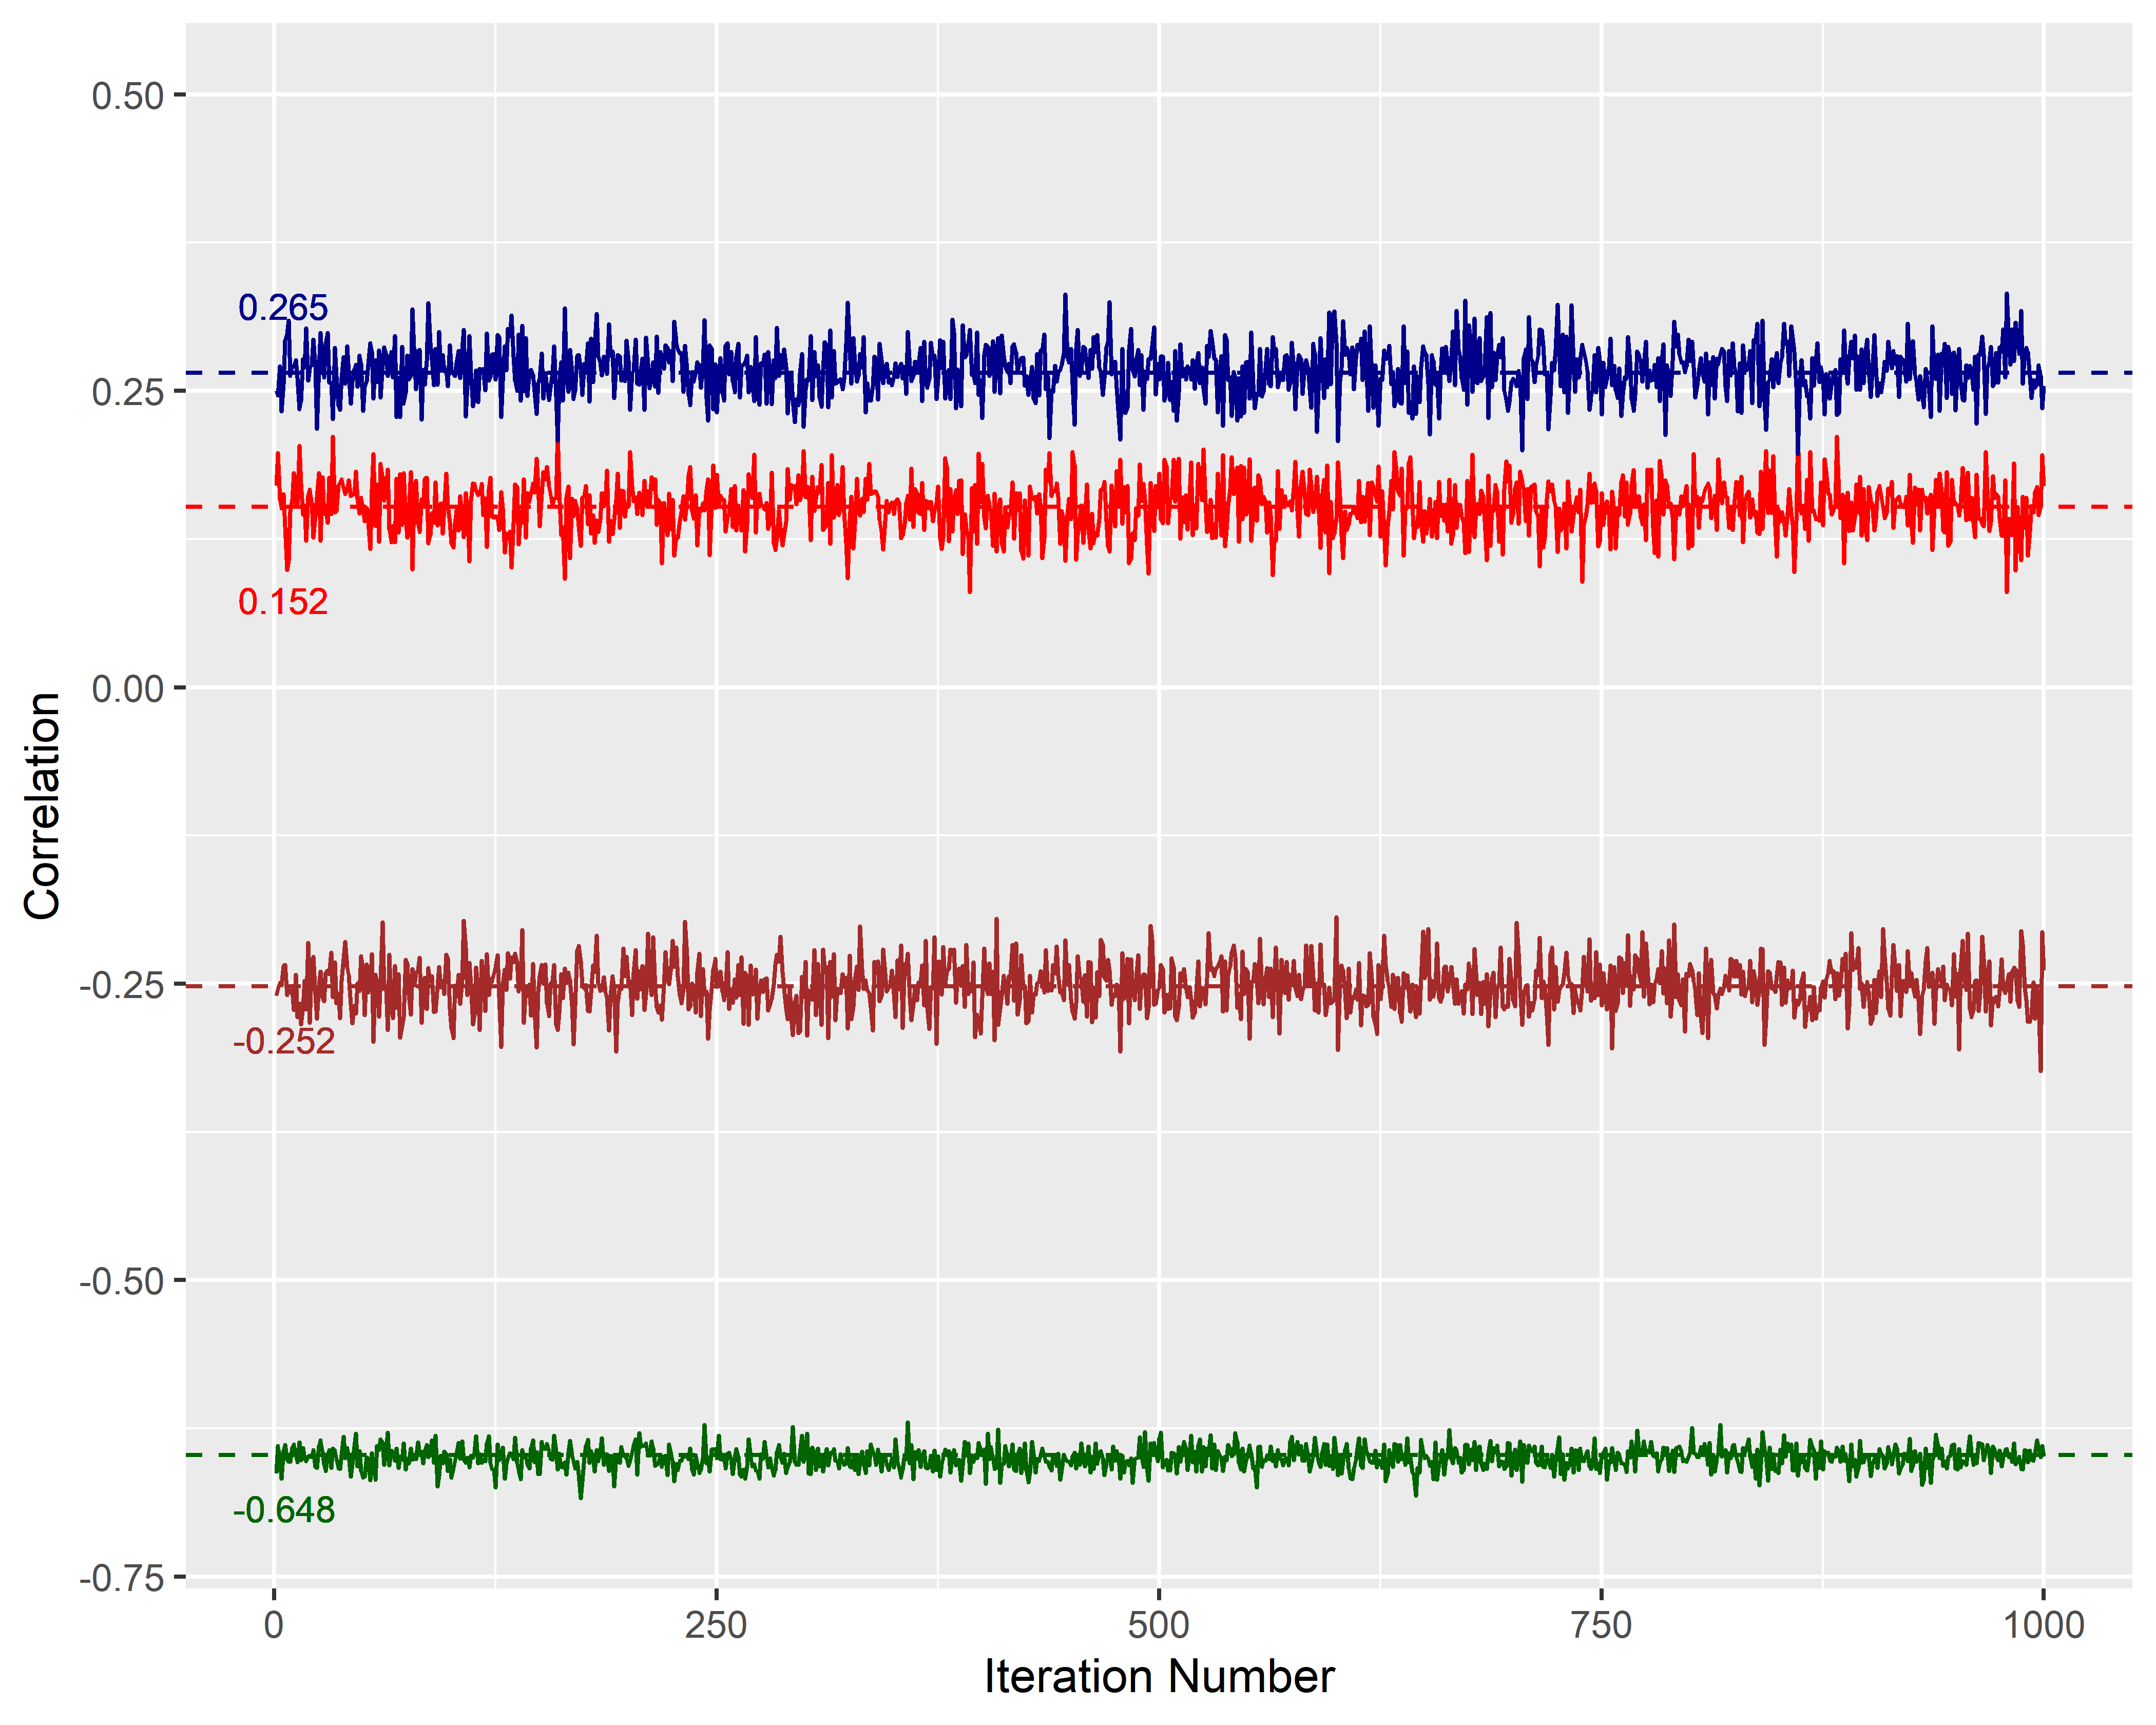
\includegraphics[width = \textwidth, height=0.8\textwidth,keepaspectratio]{artificial_alt.png}
\caption{Artificial data example: Empirical values versus specified correlations across 1,000 replications (four out of six unique pairwise correlations). Trace plot of empirical correlations that appear to closely approximate the specified correlations across 1,000 replications.}
 \label{f-1}
\end{figure}
\end{center}

To further illustrate the precision of the algorithm, we use the entries (1, 2), (1, 3), (2, 3), (3, 4) of the empirical correlation matrices to generate the plot as shown in Figure \ref{f-1} using the R package \CRANpkg{ggplot2} \citep{ggplot2}. The dashed lines represent the specified correlation values, the figure shows that the empirical correlation values across 1,000 iterations fluctuate around the specified ones within reasonably small ranges.

\subsubsection{Epilepsy rates modeled via univariate GPD}

The epilepsy data \citep{thall1990some} available from the R package \CRANpkg{robustbase} \citep{robustbase2020} were collected from a randomized clinical trial investigating the treatment effect of an anti-epileptic drug called Progabide, which was originally conducted by \cite{Leppik1985}. In this clinical trial study, 59 patients suffering from simple or complex partial seizures were randomized to groups receiving either
the anti-epileptic drug Progabide or a placebo in addition to standard chemotherapy. The baseline number of seizures occurred was measured for each patient followed by four successive post-randomization clinic visits with the number of seizures occurring over the previous two weeks reported. Although all patients were crossed over to the other treatment, we are only interested in modeling the number of seizures at baseline and the four pre-crossover follow-up responses for each patient as a realization of GPD using our package. The number of seizures that occur on a patient follows a Poisson distribution by assuming that each patient is independent of each other, and we regard them as fixed unit "intervals". In this scenario, the GPD is more appropriate than the ordinary Poisson distribution in modeling the count data since the patients generally do not exhibit the characteristics of homogeneity in real life. 

\subsubsection{Univariate GPD simulation with small sample size}

The data set has a relatively small sample size of 59, and we set the number of replications as 1,000. First, we simulate univariate GPD data based on the baseline seizure counts measured. The true rate $(\theta)$ and dispersion $(\lambda)$ parameters used to generate univariate GPD data are calculated by the method of moments in which the functions of parameters are set to equal to the moment estimates of the data. The simulation results of the five univariate GPD generation algorithms are presented in the table below:

\begin{table}[ht]
\caption{Epilepsy data (baseline seizure counts): specified and empirical parameters using the original sample size of 59.} 
\centering 
\begin{tabularx}{1.0\linewidth}{lcccccc}
\toprule
Parameters & Specified & Branching & Inversion & Build-Up & Chop-Down & Normal\\ [0.5ex] 
\midrule
Rate $(\theta)$        & 6.4904 & 6.7701 & 6.7548 & 6.8478 & 6.8594 & 7.9017 \\
Dispersion $(\lambda)$ & 0.7921 & 0.7817 & 0.7821 & 0.7773 & 0.7770 & 0.7597 \\
\bottomrule
\end{tabularx}
\label{t-3e}
\end{table}

The first column lists the true values of rate and dispersion parameters calculated by the method of moments. Overall, the empirical rate parameters overestimate the true rate parameters, and the empirical dispersion parameters underestimate the true dispersion parameters. We note that the \textit{Normal Approximation} method performs badly, perhaps due to the limitation of its approximation to the Poisson distribution with a small rate parameter.


\subsubsection{Estimation problems caused by simulating GPD data using a small sample size}

We can infer from the above simulation results that $\hat{\theta}$ and $\hat{\lambda}$ calculated using each of the five univariate approaches overestimates and underestimates the true $\theta$ and true $\lambda$, respectively, under a small sample size scenario. This behavior of the estimators can be explained by a close examination of the Equation (\ref{eq-1}): 

$$
\theta = \sqrt{\frac{\mu^3}{\sigma^2}}, \ \lambda = 1 - \frac{\sqrt{\mu}}{\sigma}.
$$ 

Since under a small sample size, the sample variance $\hat{\sigma^2}$ underestimates the true variance $\sigma^2$. Assuming that $\hat{\mu}$ is a consistent estimator of $\mu$, $\hat{\theta} = \sqrt{\frac{\hat{\mu}^3}{\hat{\sigma^2}}}$ overestimates the true $\theta$, and $\hat{\lambda} = 1 - \frac{\sqrt{\hat{\mu}}}{\hat{\sigma}}$ underestimates the true $\lambda$.

\subsection{Univariate GPD simulation with large sample size}

To alleviate this over/under estimation problem and demonstrate the performance of our package, we use the true $\theta$ and $\lambda$ parameters calculated from the epilepsy baseline seizure counts data to set up a new simulation scenario where the sample size is increased from 59 to 2,000 while maintaining the original distributional properties. The simulation results under this scenario are shown in the Table \ref{t-3e2} below:

\begin{table}[ht]
\caption{Epilepsy data  (baseline seizure counts): specified and empirical parameters using an augmented sample size of 2,000.} 
\centering
\begin{tabularx}{1.0\linewidth}{lcccccc} 
\toprule
Parameters & Specified & Branching & Inversion & Build-Up & Chop-Down & Normal\\ [0.5ex] 
\midrule
Rate $(\theta)$        & 6.4904 & 6.4973 & 6.4953 & 6.6879 & 6.7043 & 7.8181 \\
Dispersion $(\lambda)$ & 0.7921 & 0.7919 & 0.7920 & 0.7845 & 0.7841 & 0.7619 \\
\bottomrule
\end{tabularx}
\label{t-3e2} 
\end{table}

We note that the \textit{Build-up} and \textit{Chop-Down} methods do not work as well as the \textit{Branching} and \textit{Inversion} methods, which capture the true rate and dispersion parameters of the data. The \textit{Normal Approximation} method still does not perform well in the large sample scenario.

\subsection{Physician visits modeled via multivariate GPD}

\cite{deb1997demand} conducted research on 4,406 individuals, aged 66 and over, who are covered by Medicare (a public insurance program). The data are available as \code{DebTrivedi.rda} in the R package \CRANpkg{MixAll} \citep{MixAll2019}. For this data set, we consider the multivariate generation of two mutually exclusive measures of utilization variables, one pathologic variable, and one demographic variable: visits to a physician in an office setting (OFP), visits to a physician in a hospital outpatient setting (OPP) adjusted by adding 1 to avoid computational complexities, the number of chronic diseases and conditions (NUMCHRON), and the years of education received (SCHOOL). The simulation results based on 1,000 replications are shown below:

\begin{table}[ht]
\caption{DebTrivedi data: specified and empirical $\theta$'s and $\lambda$'s for four marginals.}
\centering 
\begin{tabularx}{0.63\paperwidth}{lccccc} 
\toprule
Parameter & Comparison & OFP & SCHOOL & OPP + 1 & NUMCHRON \\ [0.5ex] 
\midrule
& Specified & 2.0529 & 8.8291 & 0.6342 & 1.4188 \\ [-1ex]
\raisebox{1.5ex}{Rate ($\theta$)} 
& Empirical & 2.0545 & 8.8345 & 0.6357 & 1.4191 \\
\midrule
& Specified & 0.6445 & 0.1420 & 0.6378 & 0.0799 \\ [-1ex]
\raisebox{1.5ex}{Dispersion ($\lambda$)} 
& Empirical & 0.6442 & 0.1416 & 0.6373 & 0.0801 \\
\bottomrule
\end{tabularx}
\label{t-7}
\end{table}

\begin{table}[H]
\caption{DebTrivedi data: specified and empirical correlation matrices.}
\centering 
\begin{tabular}{lccccc} 
\toprule
Specified  & $Y1$ & $Y2$ & $Y3$ & $Y4$
\\ [0.5ex]
\midrule
$Y1$ & 1.0000 & 0.0644 & 0.0681 & 0.2619 \\ 

$Y2$ & 0.0644 & 1.0000 & -0.0122 & -0.0658 \\

$Y3$ & 0.0681 & -0.0122 & 1.0000 & 0.1008 \\

$Y4$ & 0.2619 & -0.0658 & 0.1008 & 1.0000 \\

\midrule

Empirical & $Y1$ & $Y2$ & $Y3$ & $Y4$ \\ [0.5ex]
\midrule
$Y1$ & 1.0000 & 0.0646 & 0.0743 & 0.2688 \\

$Y2$ & 0.0646 & 1.0000 & -0.0120 & -0.0660 \\

$Y3$ & 0.0743 & -0.0120 & 1.0000 & 0.1066 \\

$Y4$ & 0.2688 & -0.0660 & 0.1066 & 1.0000 \\
[0.5ex]
\bottomrule
\end{tabular}
\end{table}

\begin{longtable}[htbp]{lccccc} 
\caption{DebTrivedi data: specified and empirical moments.} \\
\toprule
Moments & Comparison & OFP & SCHOOL & OPP + 1 & NUMCHRON
\\ [0.5ex]
\midrule
\endfirsthead
\toprule
Moments & Comparison & OFP & SCHOOL & OPP + 1 & NUMCHRON
\\ [0.5ex]
\midrule
\endhead
&Specified & 5.7744 & 10.2903 & 1.7508 & 1.5420 \\[-1ex]
\raisebox{1.5ex}{Mean$(\mu)$} 
&Empirical & 5.7745 & 10.2922 & 1.7528 & 1.5427 \\
[0.5ex]\midrule
& Specified & 45.6871 & 13.9781 & 13.3426 & 1.8215 \\[-1ex]
\raisebox{1.5ex}{Variance$(\sigma^2)$} 
& Empirical & 45.6190 & 13.9688 & 13.3244 & 1.8231  \\
[0.5ex]\midrule
& Specified & 2.6794 & 0.4665 & 4.7475 & 1.0152 \\[-1ex]
\raisebox{1.5ex}{Skewness$(\nu_1)$} 
& Empirical & 2.6767  & 0.4660 & 4.7371 & 1.0155 \\
[0.5ex]\midrule
&Specified & 11.8495 & 0.2979 &  37.1841 & 1.2852 \\[-1ex]
\raisebox{1.5ex}{Kurtosis$(\nu_2)$} 
& Empirical & 11.8255 & 0.2972 & 37.0193 & 1.2865 \\[0.5ex]
\bottomrule
\label{tab:PPer}
\end{longtable}


\begin{table}[t]
\caption{DebTrivedi data: per cent difference between empirical and specified moments.} 
\centering 
\begin{tabularx}{0.75\linewidth}{lccccc} 
\toprule
Moments & OFP & SCHOOL & OPP + 1 & NUMCHRON \\ [0.5ex] 
\midrule
Mean $(\mu)$ & 0.00\% & 0.02\% & 0.11\% & 0.05\% \\
Variance $(\sigma^2)$ & 0.15\% &0.07\% &0.14\% &0.09\% \\
Skewness $(\nu_1)$ & 0.10\% & 0.11\% & 0.22\% & 0.03\% \\
Kurtosis $(\nu_2)$ & 0.20\% & 0.26\% & 0.44\% & 0.09\% \\
\bottomrule
\end{tabularx}
\label{t-3f} 
\end{table}

\begin{center}
\begin{figure}[H]
 \centering
 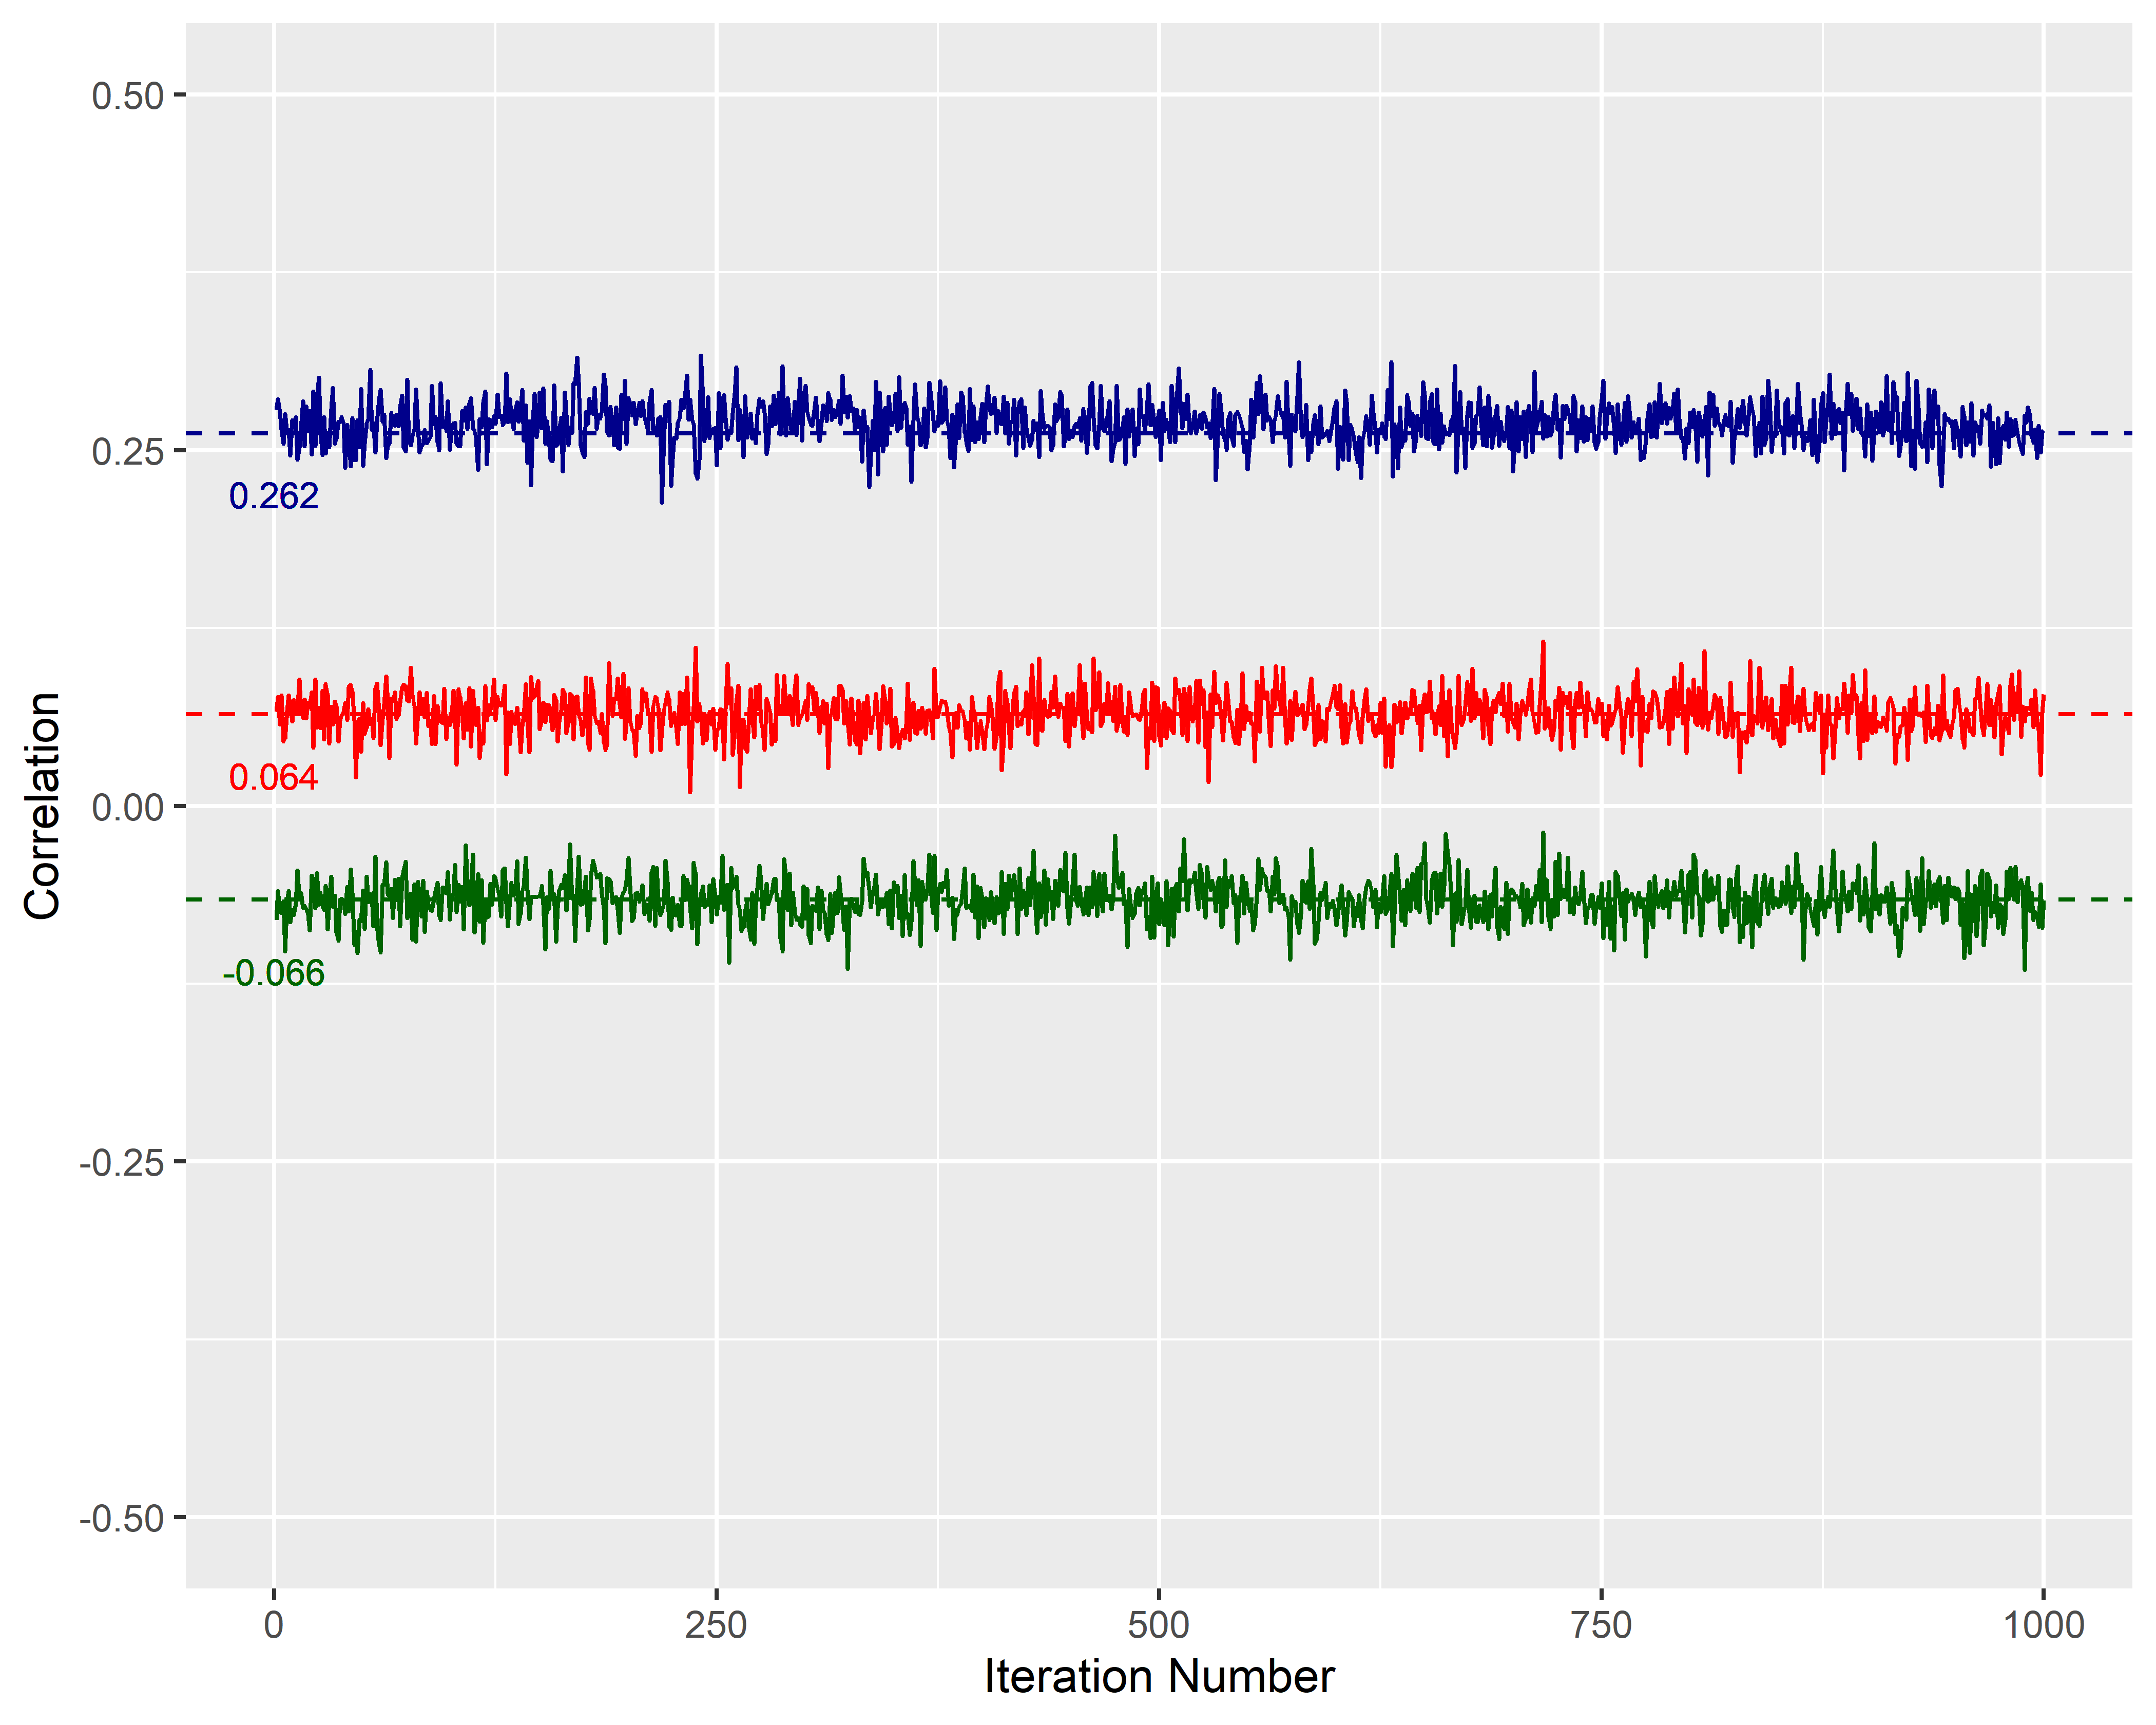
\includegraphics[width = \textwidth,height=0.8\textwidth,keepaspectratio]{DebTrivedi_alt.png}
\caption{DebTrivedi data example: Empirical values versus specified correlations across 1,000 replications (three out of six unique pairwise correlations). Trace plot of empirical correlations that appear to closely approximate the specified correlations across 1,000 replications.}
\label{f-2}
\end{figure}
\end{center}

Graphical tools further verify the simulation results: In Figure \ref{f-2}, we see that a few randomly selected empirical correlations (entries (1, 2), (1, 4), (2, 4)) across 1,000 replications fluctuate around the specified quantities within reasonably small ranges, suggesting that the algorithm is consistent and efficient in capturing the desired values.

We evaluate the performance of the package through a comparison between the theoretical and empirical first four moments and parameters, as we reported earlier in the manuscript. As correctly indicated by a reviewer, an additional assessment that involves identifying the proximity between theoretical and empirical pmf's may provide further support for the software tool under consideration. In this spirit, we show two plots (Figure \ref{fig:marginal} and Figure \ref{fig:4}) that visually validate the feasibility of our multivariate GPD generating algorithm. In Figure \ref{fig:marginal}, we compare the theoretical and empirical marginal probabilities using each of the four random variables specified in the artificial data example. The green and red dots represent the theoretical and empirical probabilities, respectively. The theoretical probabilities are calculated based on the pmf of each univariate GPD when its rate and dispersion parameters are specified. The empirical probabilities are marginally extracted from the multivariate data simulated in the artificial data example. We observe that the empirical and theoretical probabilities align closely, which suggests that our algorithm can accurately simulate data that follow the specified GPD marginally. In Figure \ref{fig:4}, we show a comparison plot between specified and empirical correlations in an attempt to examine if our multivariate GPD generating algorithm can reasonably simulate the specified correlations. We specify a bivariate GPD using the variable 2 and variable 4, as previously defined in the artificial data example. The specified correlations range from -0.89 to 0.86 with an increasing step size of 0.05, which are within the lower and upper correlation bounds, as verified using the \code{ComputeCorrGpois} function. For each specified correlation, we generate a sample of 100 observations with 50 replications, and calculate the average empirical correlation. The plot shows that empirical correlations closely approximate the specified correlations for all scenarios.

\begin{center}
    \begin{figure}[H]
        \centering
        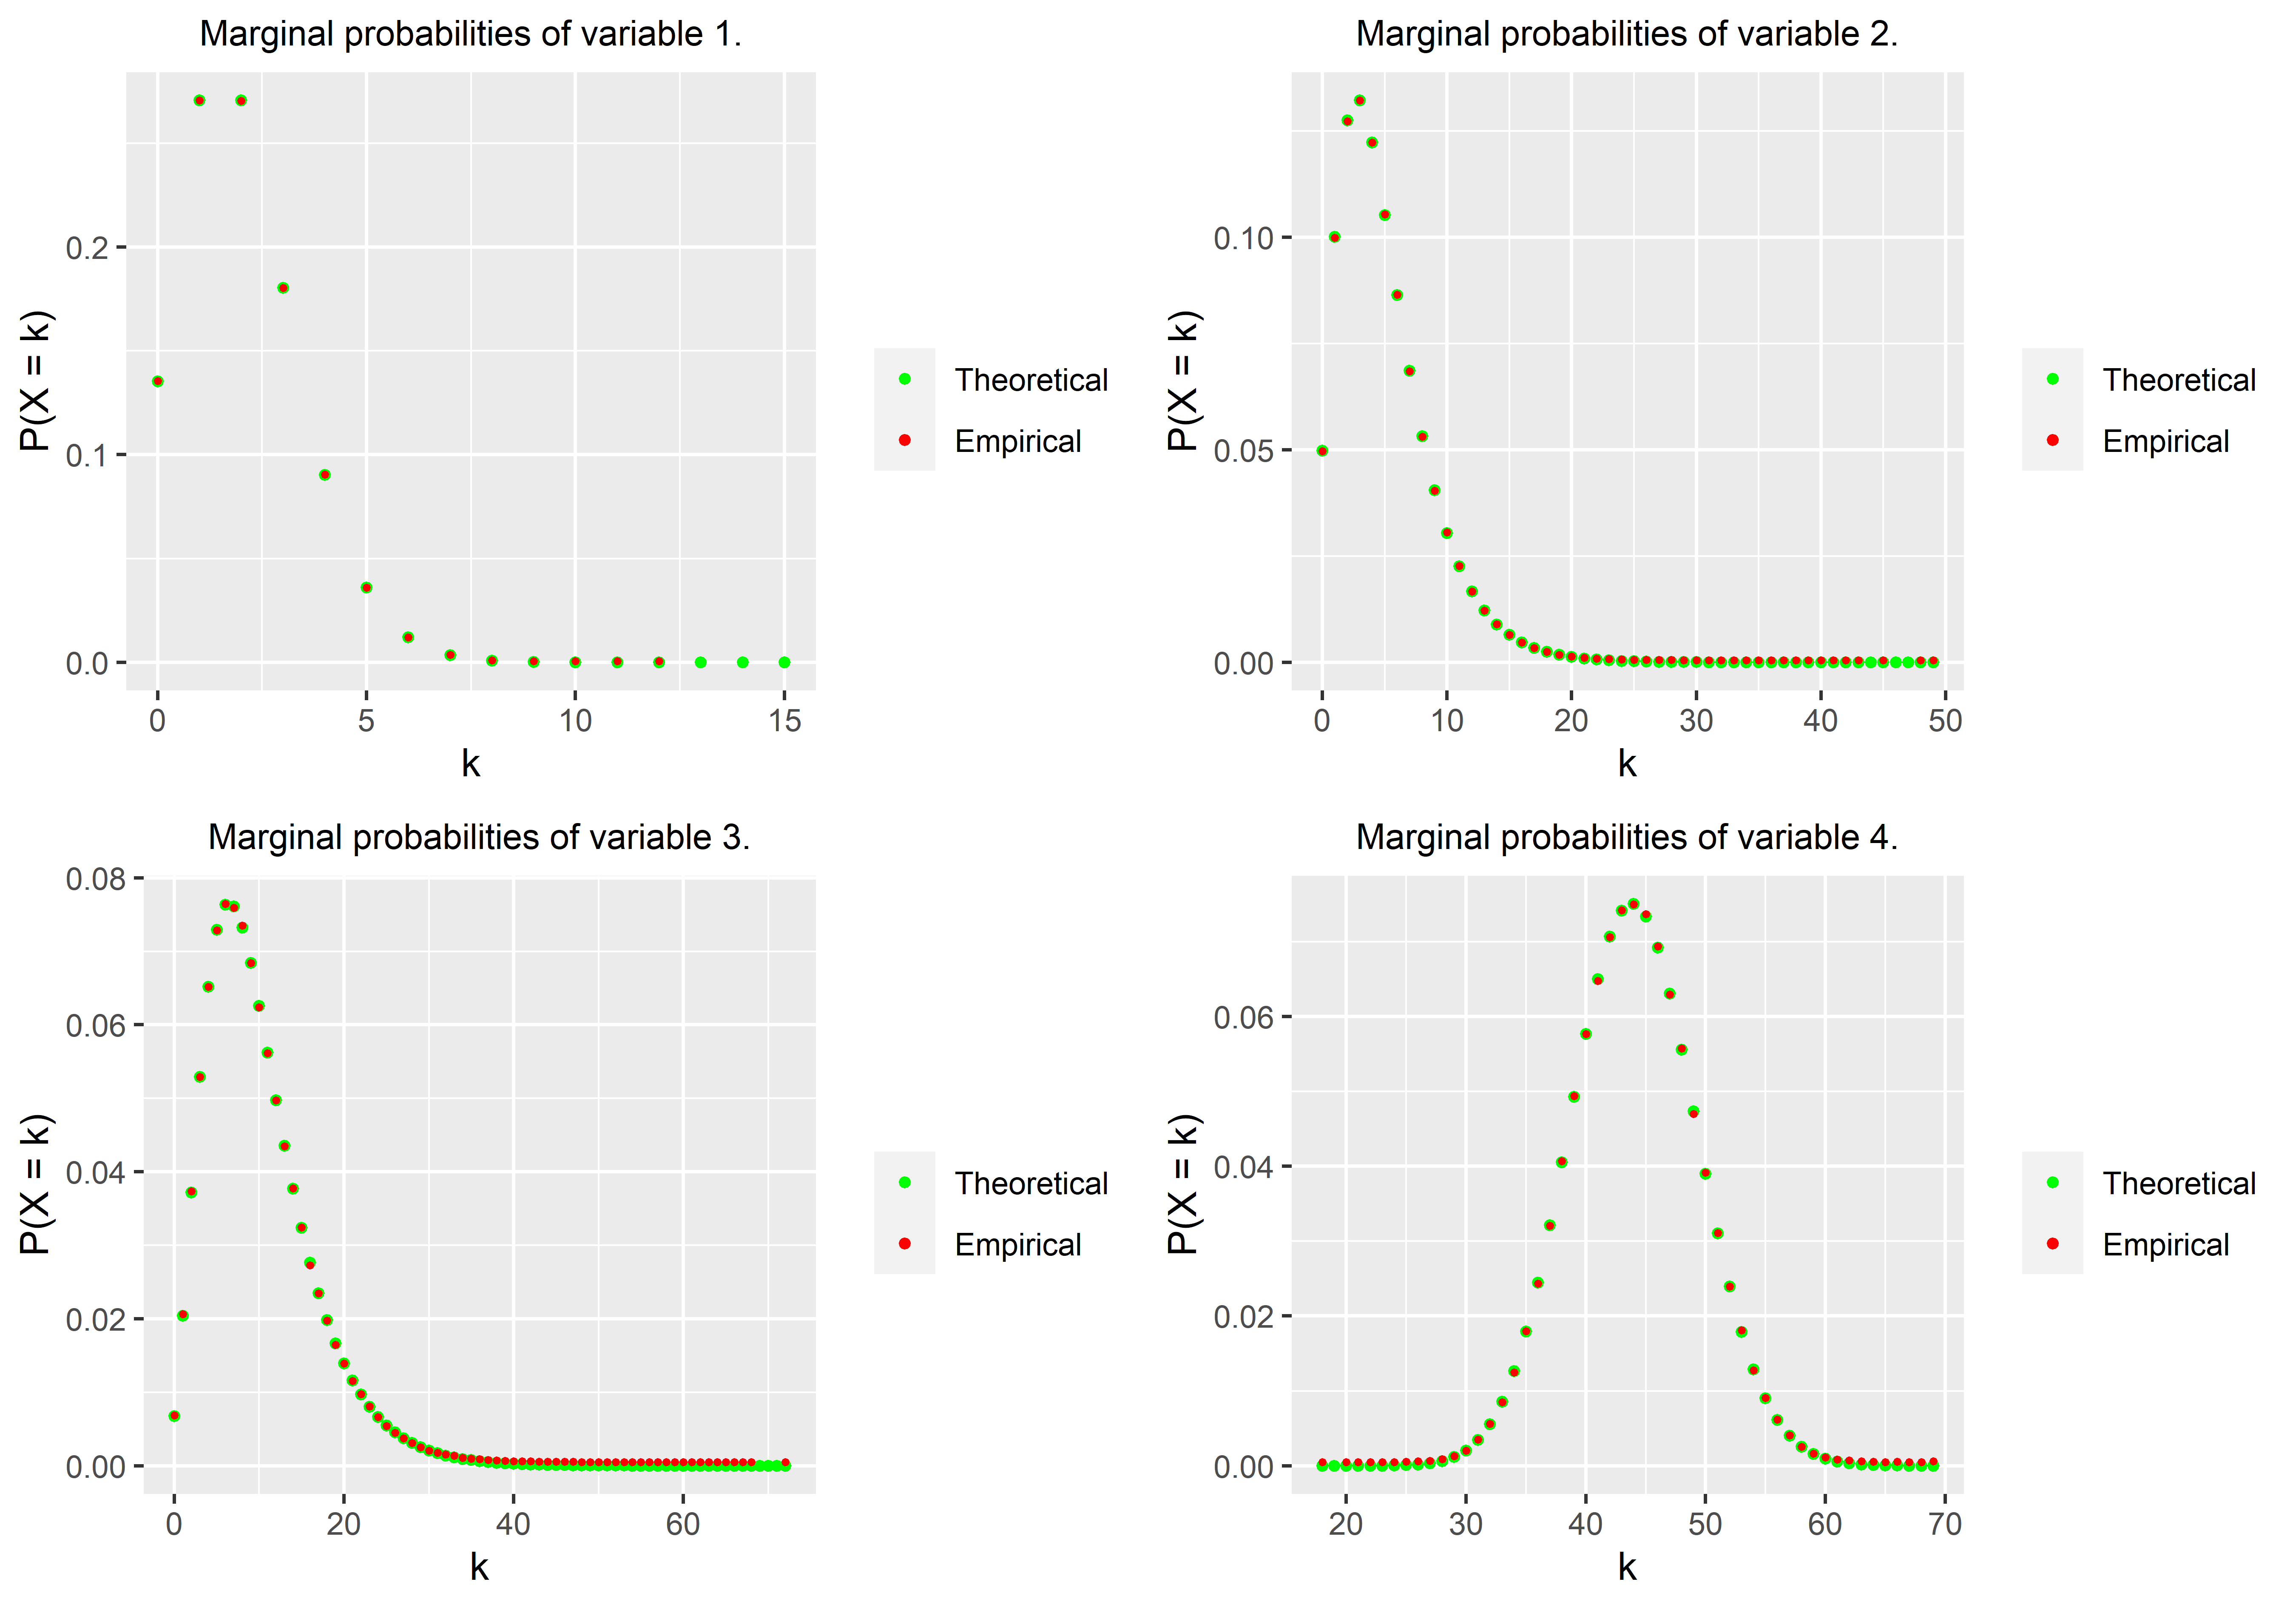
\includegraphics[width = \textwidth,height = 0.7\textwidth,keepaspectratio]{fig3_marginal_PMFs.png}
        \caption{Comparison of theoretical and empirical marginal probabilities. The plot indicates that the empirical marginal probabilities closely approximate the theoretical marginal probabilities.}
        \label{fig:marginal}
    \end{figure}
\end{center}

\begin{center}
    \begin{figure}[H]
        \centering
        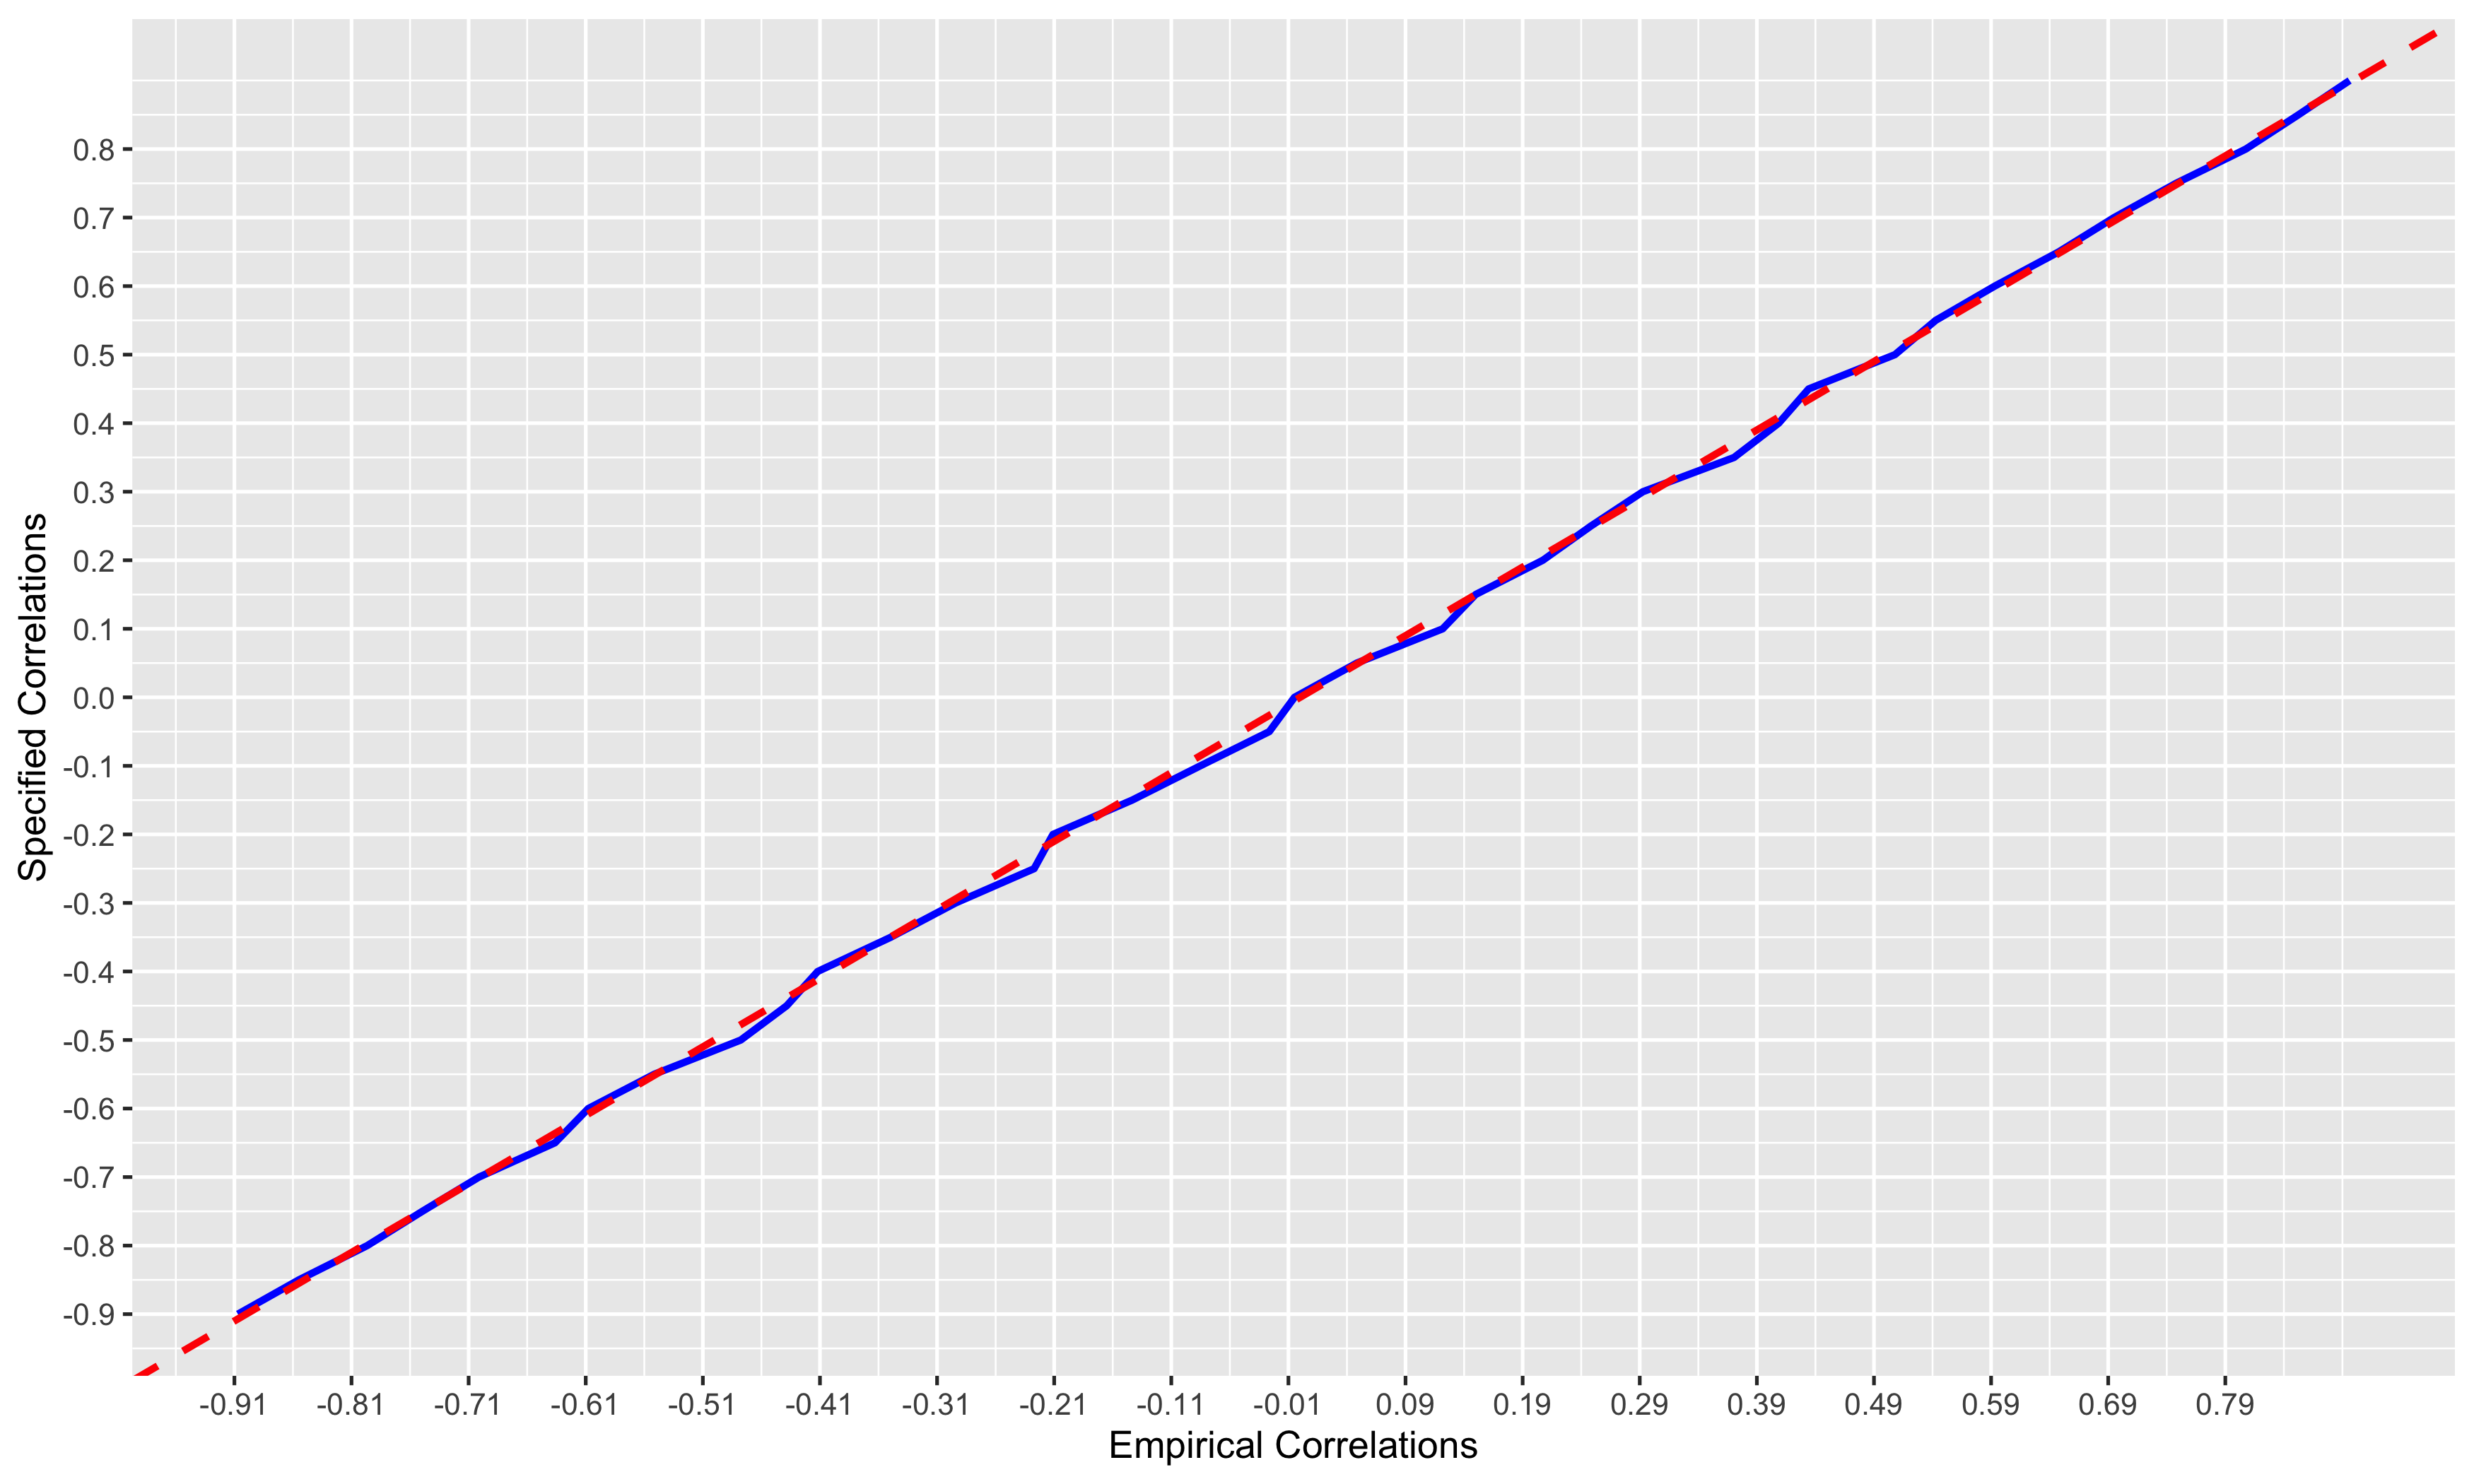
\includegraphics[width = 0.9\textwidth,height=0.7\textwidth,keepaspectratio]{fig4_samp100_iter_50_350dpi.png}
        \caption{Comparison of specified and empirical correlations. The slope of the red dashed line is one, and is used for calibration. The blue solid line represents the empirical correlations plotted against the specified correlations at varying specifications.}
        \label{fig:4}
    \end{figure}
\end{center}

\vspace*{-5mm}

\section{Discussion}

Throughout this paper, we have demonstrated the functionality and performance of the \pkg{RNGforGPD} package. This package is an accurate and computationally efficient tool in random generation of both univariate and multivariate data that follow the generalized Poisson distribution. Overall, the performance of the algorithm is decent. Deviations between the specified and average empirical parameter values are within tolerable limits in both the univariate and multivariate data generation cases. Our simulation studies suggest that this package successfully implements the algorithms in both artificial and real life scenarios as long as there are no specification errors and the correlations are within the feasible limits \citep{demirtas2011practical}. In situations such complications occur, appropriate warning or error messages will be generated to alert the user. The simulation results we present can be regarded as a compelling evidence for capturing the characteristics of both rate and dispersion parameters (naturally the first four moments that are functions of these quantities) as well as the true association structure in the multivariate cases with only minor differences. In summary, the \pkg{RNGforGPD} package provides a valuable tool for investigators who need a generalized Poisson data generation mechanism in their research.

\bibliography{RNGforGPD_paper_LDC_R_Journal}

\address{Hesen Li\\
  Ph.D. Student\\
  Division of Epidemiology and Biostatistics\\
  University of Illinois at Chicago\\
  Chicago, IL 60612, USA\\
  ORCID: 0000-0003-1636-299X\\}
\email{hli226@uic.edu}

\address{Dr. Hakan Demirtas\\
  Associate Professor of Biostatistics\\
  Division of Epidemiology and Biostatistics\\
  University of Illinois at Chicago\\
  Chicago, IL 60612, USA\\
  ORCID: 0000-0003-2482-703X\\}
\email{demirtas@uic.edu}

\address{Ruizhe Chen\\
  Ph.D. Student\\
  Division of Epidemiology and Biostatistics\\
  University of Illinois at Chicago\\
  Chicago, IL 60612, USA\\
ORCID: 0000-0003-3924-3328\\}
\email{rchen18@uic.edu}


